\section{Predicate tableau}

In first-order logic, a \emph{literal} is an atom or its negation, i.e.
%
\[r^n (t_1, t_2, \cdots, t_n)\]
or
\[\neg r^n (t_1, t_2, \cdots, t_n)\]
%
where \(r^n\) is an \(n\)-ary predicate and \(t_i\) is a term.

The method for tableau construction in first-order logic is identical to that in propositional logic, but with a few extra expansion rules for dealing with quantifiers.


\subsection{Expansion rules}

In addition to \(\alpha\)- and \(\beta\)-rules, we also require \(\delta\)- and \(\gamma\)-rules, as depicted in Figures \ref{fig:Ch04-delta-rules} and \ref{fig:Ch04-gamma-rules}.


\begin{figure}[H]
    \centering
    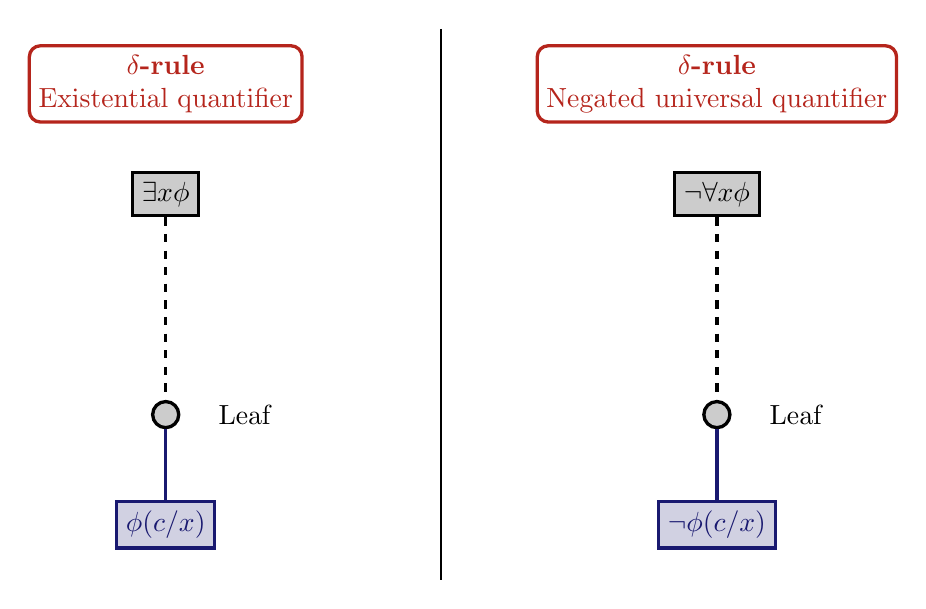
\begin{tikzpicture}[scale=1.4]
        \begin{scope}[shift={(0, 0)}]
            \node (root) at (0, 1)[draw=BrickRed, very thick, BrickRed, rounded corners, align=center] {\textbf{\(\delta\)-rule} \\ Existential quantifier};

            \node (root) at (0, 0)[draw=black, very thick, fill=black!20] {\(\exists x \phi\)};

            \node (leaf) at (0, -2)[circle, draw=black, very thick, fill=black!20] {};

            \node [right of=leaf, black] {Leaf};

            \draw[dashed, very thick] (root) -- (leaf);

            \node (child1) at (0, -3)[draw=MidnightBlue, very thick, MidnightBlue, fill=MidnightBlue!20] {\(\phi(c/ x)\)};

            \draw[very thick, MidnightBlue] (leaf) -- (child1);
        \end{scope}
        
        \begin{scope}[shift={(5, 0)}]
            \node (root) at (0, 1)[draw=BrickRed, very thick, BrickRed, rounded corners, align=center] {\textbf{\(\delta\)-rule} \\ Negated universal quantifier};

            \node (root) at (0, 0)[draw=black, very thick, fill=black!20] {\(\neg\forall x \phi\)};

            \node (leaf) at (0, -2)[circle, draw=black, very thick, fill=black!20] {};

            \node [right of=leaf, black] {Leaf};

            \draw[dashed, very thick] (root) -- (leaf);

            \node (child1) at (0, -3)[draw=MidnightBlue, very thick, MidnightBlue, fill=MidnightBlue!20] {\(\neg\phi(c/ x)\)};

            \draw[very thick, MidnightBlue] (leaf) -- (child1);
        \end{scope}

        \draw[thick] (2.5, 1.5) -- (2.5, -3.5);
    \end{tikzpicture}
    \caption{The two \(\delta\)-rules for constructing predicate tableaus. In both rules, \(c\) should be a new constant that has not been used in the tableau before.}
    \label{fig:Ch04-delta-rules}
\end{figure}


\begin{figure}[H]
    \centering
    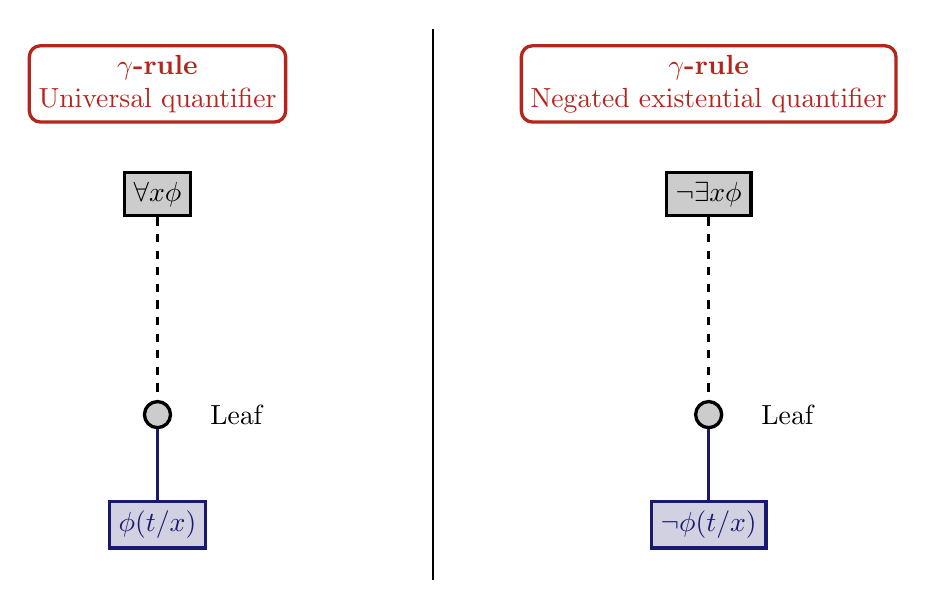
\begin{tikzpicture}[scale=1.4]
        \begin{scope}[shift={(0, 0)}]
            \node (root) at (0, 1)[draw=BrickRed, very thick, BrickRed, rounded corners, align=center] {\textbf{\(\gamma\)-rule} \\ Universal quantifier};

            \node (root) at (0, 0)[draw=black, very thick, fill=black!20] {\(\forall x \phi\)};

            \node (leaf) at (0, -2)[circle, draw=black, very thick, fill=black!20] {};

            \node [right of=leaf, black] {Leaf};

            \draw[dashed, very thick] (root) -- (leaf);

            \node (child1) at (0, -3)[draw=MidnightBlue, very thick, MidnightBlue, fill=MidnightBlue!20] {\(\phi(t/x)\)};

            \draw[very thick, MidnightBlue] (leaf) -- (child1);
        \end{scope}

        \begin{scope}[shift={(5, 0)}]
            \node (root) at (0, 1)[draw=BrickRed, very thick, BrickRed, rounded corners, align=center] {\textbf{\(\gamma\)-rule} \\ Negated existential quantifier};

            \node (root) at (0, 0)[draw=black, very thick, fill=black!20] {\(\neg\exists x \phi\)};

            \node (leaf) at (0, -2)[circle, draw=black, very thick, fill=black!20] {};

            \node [right of=leaf, black] {Leaf};

            \draw[dashed, very thick] (root) -- (leaf);

            \node (child1) at (0, -3)[draw=MidnightBlue, very thick, MidnightBlue, fill=MidnightBlue!20] {\(\neg\phi(t/ x)\)};

            \draw[very thick, MidnightBlue] (leaf) -- (child1);
        \end{scope}

        \draw[thick] (2.5, 1.5) -- (2.5, -3.5);
    \end{tikzpicture}
    \caption{The two \(\gamma\)-rules for constructing predicate tableaus. In both rules, \(t\) is a closed term. Formulas should \textbf{not} be ticked following a \(\gamma\)-rule expansion.}
    \label{fig:Ch04-gamma-rules}
\end{figure}

When applying a \(\delta\)-rule, make sure to introduce a new constant symbol that is not used anywhere before in the tableau. This new constant acts as a \emph{witness}\footnote{Or: \emph{Skolem witness}.} for the existential statement.

Compared to the other rules, \(\gamma\)-rules are usually applied last. When applying a \(\gamma\)-rule, instantiate \(x\) with a closed term that appeared earlier in the current branch\footnote{This closed term should \textbf{not} be new.}. Formulas expanded via a \(\gamma\)-rule should \textbf{not} be ticked.



\subsection{Termination}

Similar to propositional tableaus, a predicate tableau's branch is closed if it contains both a literal \(P(t_1, t_2, \cdots, t_n)\) and its negation \(\neg P(t_1, t_2, \cdots, t_n)\). Otherwise, it is open.

The tableau terminates when:
%
\begin{itemize}
    \item Every branch is closed. This shows that the root formula is unsatisfiable.
    \item All formulas are fully expanded and no further rules can be applied. If at least one branch remains open and cannot be further expanded, the tableau is open, indicating the root formula's satisfiability.
\end{itemize}




\subsection{Example}

Suppose we want to check whether the formula
%
\[(\forall x\; \neg p(x) \rightarrow \neg\exists y\; p(y))\]
%
is valid. To do this, we place its negation at the root of our tableau.


\begin{figure}[H]
    \centering
    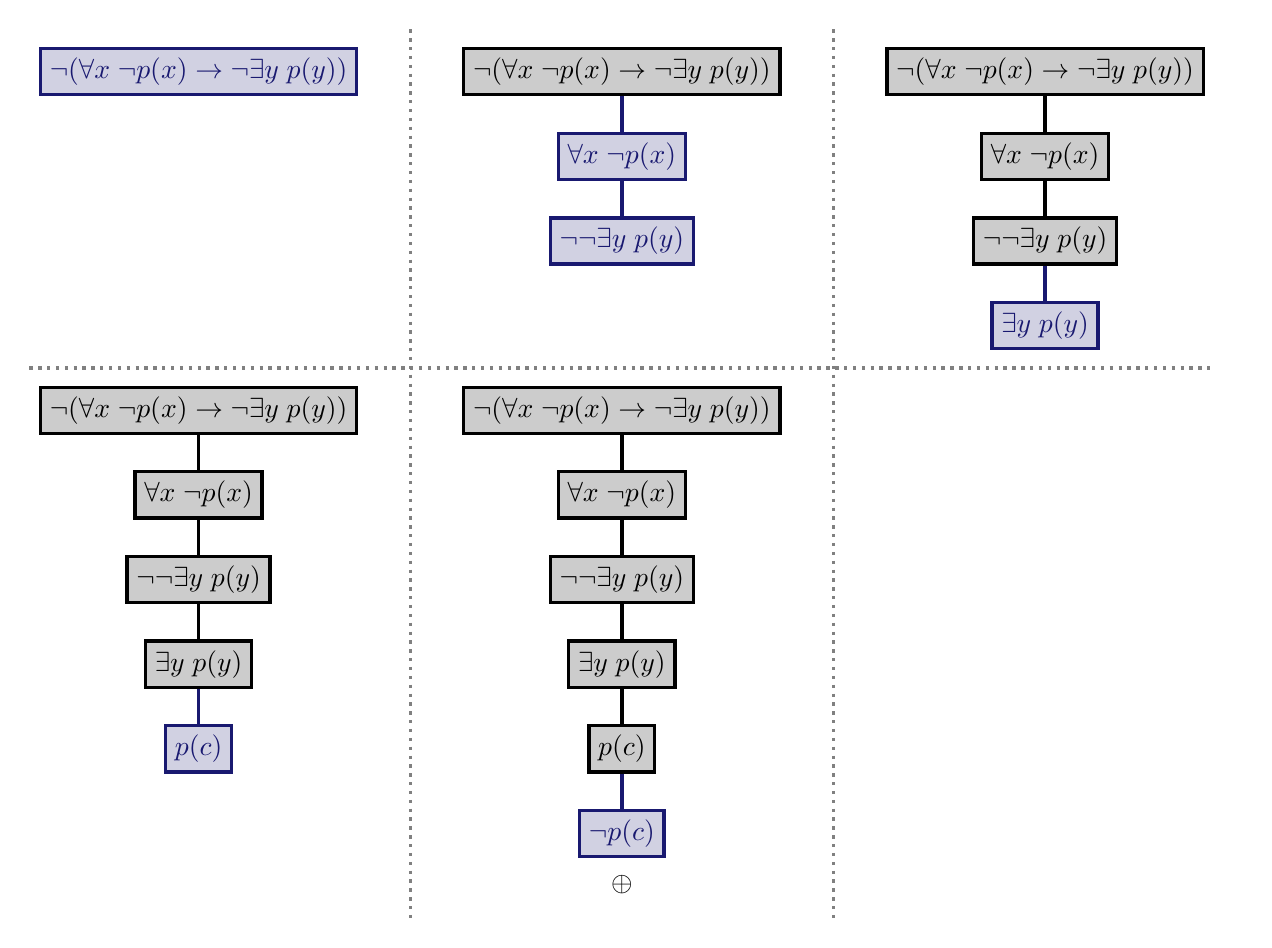
\begin{tikzpicture}[scale=1.075]
        \begin{scope}[shift={(0, 0)}]
            \node (0) at (0, 0)[draw=MidnightBlue, very thick, MidnightBlue, fill=MidnightBlue!20] {\(\neg(\forall x\; \neg p(x) \rightarrow \neg\exists y\; p(y))\)};
        \end{scope}

        \begin{scope}[shift={(5, 0)}]
            \node (0) at (0, 0)[draw=black, very thick, fill=black!20] {\(\neg(\forall x\; \neg p(x) \rightarrow \neg\exists y\; p(y))\)};
            \node[right of=0, xshift=40pt] {\checkmark};

            \node (1) at (0, -1)[draw=MidnightBlue, very thick, MidnightBlue, fill=MidnightBlue!20] {\(\forall x\; \neg p(x)\)};

            \node (2) at (0, -2)[draw=MidnightBlue, very thick, MidnightBlue, fill=MidnightBlue!20] {\(\neg\neg\exists y\; p(y)\)};

            \draw[MidnightBlue, very thick] (0) -- (1) -- (2);
        \end{scope}

        \begin{scope}[shift={(10, 0)}]
            \node (0) at (0, 0)[draw=black, very thick, fill=black!20] {\(\neg(\forall x\; \neg p(x) \rightarrow \neg\exists y\; p(y))\)};
            \node[right of=0, xshift=40pt] {\checkmark};

            \node (1) at (0, -1)[draw=black, very thick, fill=black!20] {\(\forall x\; \neg p(x)\)};

            \node (2) at (0, -2)[draw=black, very thick, fill=black!20] {\(\neg\neg\exists y\; p(y)\)};
            \node[right of=2, xshift=10pt] {\checkmark};

            \node (3) at (0, -3)[draw=MidnightBlue, very thick, MidnightBlue, fill=MidnightBlue!20] {\(\exists y\; p(y)\)};

            \draw[black, very thick] (0) -- (1) -- (2);
            \draw[MidnightBlue, very thick] (2) -- (3);
        \end{scope}

        \begin{scope}[shift={(0, -4)}]
            \node (0) at (0, 0)[draw=black, very thick, fill=black!20] {\(\neg(\forall x\; \neg p(x) \rightarrow \neg\exists y\; p(y))\)};
            \node[right of=0, xshift=40pt] {\checkmark};

            \node (1) at (0, -1)[draw=black, very thick, fill=black!20] {\(\forall x\; \neg p(x)\)};

            \node (2) at (0, -2)[draw=black, very thick, fill=black!20] {\(\neg\neg\exists y\; p(y)\)};
            \node[right of=2, xshift=10pt] {\checkmark};

            \node (3) at (0, -3)[draw=black, very thick, fill=black!20] {\(\exists y\; p(y)\)};
            \node[right of=3] {\checkmark};

            \node (4) at (0, -4)[draw=MidnightBlue, very thick, MidnightBlue, fill=MidnightBlue!20] {\(p(c)\)};

            \draw[black, very thick] (0) -- (1) -- (2) -- (3);
            \draw[MidnightBlue, very thick] (3) -- (4);
        \end{scope}

        \begin{scope}[shift={(5, -4)}]
            \node (0) at (0, 0)[draw=black, very thick, fill=black!20] {\(\neg(\forall x\; \neg p(x) \rightarrow \neg\exists y\; p(y))\)};
            \node[right of=0, xshift=40pt] {\checkmark};

            \node (1) at (0, -1)[draw=black, very thick, fill=black!20] {\(\forall x\; \neg p(x)\)};

            \node (2) at (0, -2)[draw=black, very thick, fill=black!20] {\(\neg\neg\exists y\; p(y)\)};
            \node[right of=2, xshift=10pt] {\checkmark};

            \node (3) at (0, -3)[draw=black, very thick, fill=black!20] {\(\exists y\; p(y)\)};
            \node[right of=3] {\checkmark};

            \node (4) at (0, -4)[draw=black, very thick, fill=black!20] {\(p(c)\)};

            \node (5) at (0, -5)[draw=MidnightBlue, very thick, MidnightBlue, fill=MidnightBlue!20] {\(\neg p(c)\)};
            \node [below of=5, yshift=10pt] {\(\oplus\)};

            \draw[black, very thick] (0) -- (1) -- (2) -- (3) -- (4);
            \draw[MidnightBlue, very thick] (4) -- (5);
        \end{scope}

        \draw[gray, very thick, dotted] (2.5, 0.5) -- (2.5, -10);
        \draw[gray, very thick, dotted] (7.5, 0.5) -- (7.5, -10);
        \draw[gray, very thick, dotted] (-2, -3.5) -- (12, -3.5);
    \end{tikzpicture}
    \caption{Constructing the tableau of \(\neg(\forall x\; \neg p(x) \rightarrow \neg\exists y\; p(y))\). Read from left to right and from top to bottom. In the fourth step (bottom left), the existential formula \(\exists y\; p(y)\) is expanded via a \(\delta\)-rule by introducing a new constant \(c\). In the last step (bottom middle), the universal formula \(\forall x\; \neg p(x)\) is expanded via a \(\gamma\)-rule by replacing all bounded instances of \(x\) with the closed term \(c\) from earlier in the current branch, thereby producing both \(p(c)\) and \(\neg p(c)\) in the same branch. This results in a closed branch and hence a closed tableau, indicating that the formula at the root is unsatisfiable.}
    \label{fig:Ch04-satisfiability-tableau}
\end{figure}

As shown, the negation \(\neg(\forall x\; \neg p(x) \rightarrow \neg\exists y\; p(y))\) is unsatisfiable. This means that our original formula must be valid.




\subsection{Non-termination}

Predicate tableaus may not always terminate.

For instance, if a tableau unendingly generates nodes that require expansion via \(\delta\)-rules, more and more constants would be introduced, and the number of \(\gamma\)-rule applications required would increase dramatically. This may result in non-termination.

Before we elaborate on this non-terminating scenario, we must note that in order to systematically handle possible infinite expansions, we should adopt a fair application strategy. A tableau construction is \emph{fair} if
%
\begin{itemize}
    \item Every formula that can still be expanded eventually will be, and
    \item Every formula that falls under a \(\gamma\)-rule will eventually be instantiated via that rule using all closed terms that appear in its branch.
\end{itemize}
%
This ensures that if the tableau can close, it will close after finitely many steps. We won't miss a contradiction because we ignored a rule.

Now, assuming a fair application strategy,
%
\begin{itemize}
    \item If a branch keeps repeating the same configuration of formulas over and over with no new information, it is effectively saturated. This branch is then considered open, meaning that the root formula is satisfiable. This is because we may construct an infinite model for the root formula by reading off literals in the limit of the infinitely ``looping'' branch in the same way as we did for propositional tableaus. See Figure \ref{fig:Ch04-non-terminating-tableau} for an example.
    \item If a branch runs indefinitely without closure, the satisfiability of the root formula is \textbf{undecided} and \textbf{inconclusive}.
\end{itemize}


\begin{figure}[H]
    \centering
    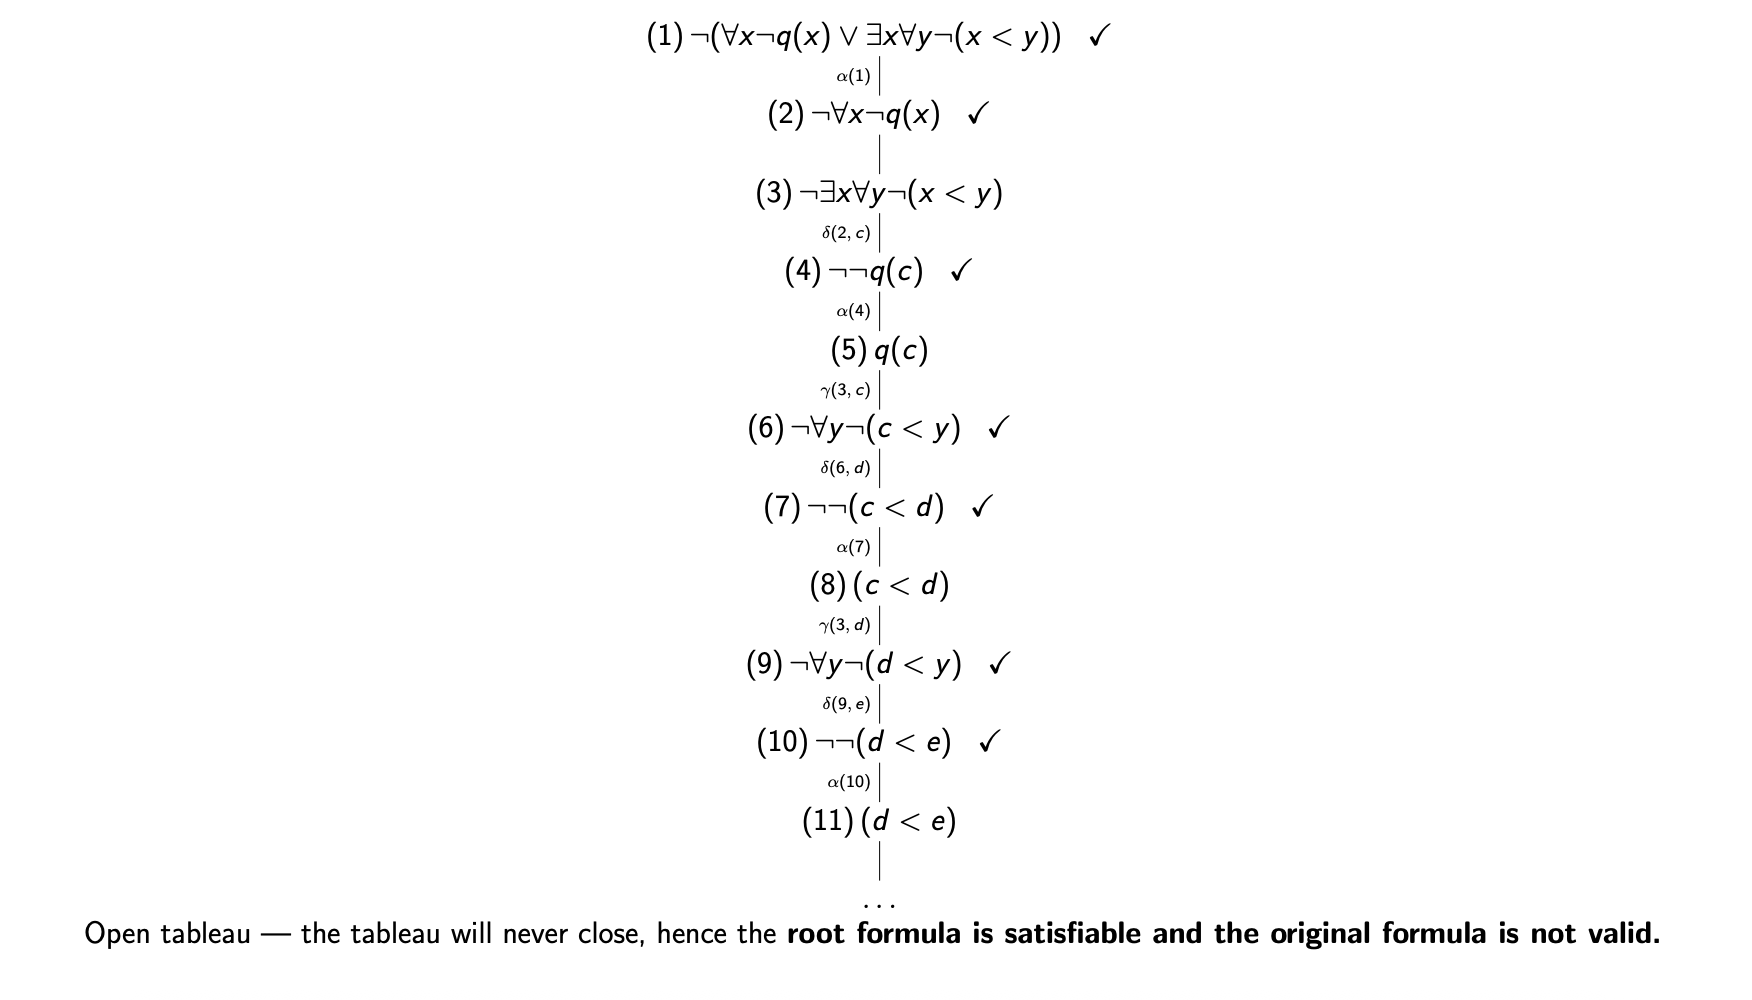
\includegraphics[width=0.95\textwidth]{Images/04a_NonterminatingPredicateTableau.png}
    \caption{A non-terminating tableau where the root formula is satisfiable.}
    \label{fig:Ch04-non-terminating-tableau}
\end{figure}



\subsection{Free variables}

Predicate tableaus are predominantly designed to work on sentences, where free variables are not allowed. To prove the validity of a formula with free variables, we may prefix it with an appropriate universal quantifier. For instance, if we want to show that
%
\[x < 5\]
%
is valid, where \(x\) is a free variable. Notice that this is equivalent to showing the validity of
%
\[\forall x\; x < 5\]
%
which uses a universal quantifier to remove the free variable. Consequently, we can simply construct a tableau with
%
\[\neg\forall x\; x < 5\]
%
at its root and check its satisfiability as usual.



\subsection{More on fairness}

Note that when applying expansion rules in non-terminating predicate tableaus, it is always possible to find a fair application strategy.

To see why this is, consider a countably infinite set of processes \(P = \{P_1, P_2, \cdots, P_i, \cdots\}\), each awaiting some input. When a process receives an input, this may result in the creation of a new process, which is subsequently added to \(P\). We want to find some fair schedule where if any process \(P_i\) is awaiting input at time \(t\), then eventually at some time \(t' > t\) it will receive some input.

Since the set \(P\) always remains countable even when a new process is created and added to it, such a schedule must exist.